\chapter{Installation et premiers conseils}

\section{Principes généraux}

Pour utiliser \LaTeX{}, il faut installer, dans l'ordre,

$\star$ une distribution

$\star$ un éditeur de textes

On tape un document appelé \jargon{code source} dans l'éditeur de textes et on l'enregistre au format \texttt{.tex}.

On \jargon{compile} ce document pour obtenir un document lisible, en général au format \texttt{.pdf}. La compilation utilise la distribution \LaTeX{} que vous avez installée.

Lors de l'installation d'une distribution, je vous conseille d'effectuer une installation complète de la distribution, c'est-à-dire avec tous les \jargon{packages}.

Mais si malgré cela, il vous manque des \jargon{packages}, vous les trouverez directement sur le site de l'auteur du \jargon{package} et sur la \og banque des \jargon{packages} \LaTeX{} \fg{} : \url{https://www.ctan.org/}.

En général, l'auteur du \jargon{package} fournit une notice de ce \jargon{package} et on retrouve cette notice sur le site \url{https://www.ctan.org/}.

Si vous souhaitez ajouter un \jargon{package} à votre distribution, reportez vous à la dernière section de ce chapitre.



\section{Les distributions}

Il existe des distributions \LaTeX{} pour \jargon{Linux}, \jargon{Windows} ou \jargon{Mac}.

La distribution \jargon{TeXLive} existe pour \jargon{Linux} et \jargon{Windows}.

La distribution \jargon{MiKTeX} est une distribution uniquement pour \jargon{Windows}.

La distribution \jargon{MacTeX} est une distribution uniquement pour \jargon{Mac}.

Personnellement, j'utilise la distribution \jargon{TeXLive} sur \jargon{Linux} et \jargon{Windows}.

L'installation de ces distributions est très bien détaillée sur le site 

\url{http://www.xm1math.net/doculatex/index.html}.

Pour ceux qui souhaitent installer \jargon{TeXLive} mais n'ont pas de DVD sous la main, comme indiqué sur le site précédent, il existe d'autres possibilités :

$\star$ installation à partir du site \url{http://tug.org/texlive/acquire-netinstall.html} (en Anglais)

$\star$ utilisation du logiciel \jargon{Daemon Tools} qui permet, sous \jargon{Windows}, à partir d'une image \texttt{.iso} de créer un DVD virtuel

$\star$ ou montage, sous \jargon{Linux} de l'image \texttt{.iso}

\section{\'Editeurs de textes}

On peut utiliser n'importe quel éditeur de textes pour utiliser \LaTeX{}. Il suffit d'enregistrer le \jargon{fichier source} avec comme extension \texttt{.tex}.

Mais, je vous conseille d'utiliser un éditeur de textes spécifique à \LaTeX{}.

Il en existe plusieurs, dont, par exemple \jargon{TeXmaker} ou \jargon{TeXStudio}.

Personnellement, j'utilise le premier des deux qui fonctionne sous toutes les plateformes (\jargon{Linux}, \jargon{Windows} ou \jargon{Mac}).

Un éditeur spécifique à \LaTeX{} vous permettra, entre autres\dots

$\star$ d'avoir le \jargon{code source} colorié automatiquement en fonction des commandes que vous utiliser,

$\star$ d'utiliser l'auto-complétion pour les commandes usuelles de \LaTeX{},

$\star$ d'ajouter d'autres commandes (y compris celles que vous avez créées) dans le \og vocabulaire \fg{} du logiciel et ainsi utiliser l'auto-complétion pour ces commandes,

$\star$ de créer des raccourcis clavier pour des bouts de code que vous utilisez souvent,

$\star$ de paramétrer de différentes façons la compilation de votre document.

L'installation de \jargon{TeXmaker} est détaillée sur le site précédent :

\url{http://www.xm1math.net/doculatex/index.html}

\medskip

\textbf{Remarque :}

Il existe également des éditeurs en ligne (dans un navigateur) qui ont l'avantage de pouvoir compiler le document au fur et à mesure qu'on le tape.

On peut utiliser par exemple \url{https://www.overleaf.com/} qui est un très bon éditeur en ligne.

Il suffira alors de créer un compte gratuitement pour pouvoir créer des documents avec un espace de 100 Mb au départ.

\section{Afficher le fichier .pdf obtenu après compilation dans TexMaker}

On suit les étapes suivantes :

$\star$ Dans le menu \og Options \fg{}, on clique sur \og Configurer Texmaker \fg{} :
\begin{center}
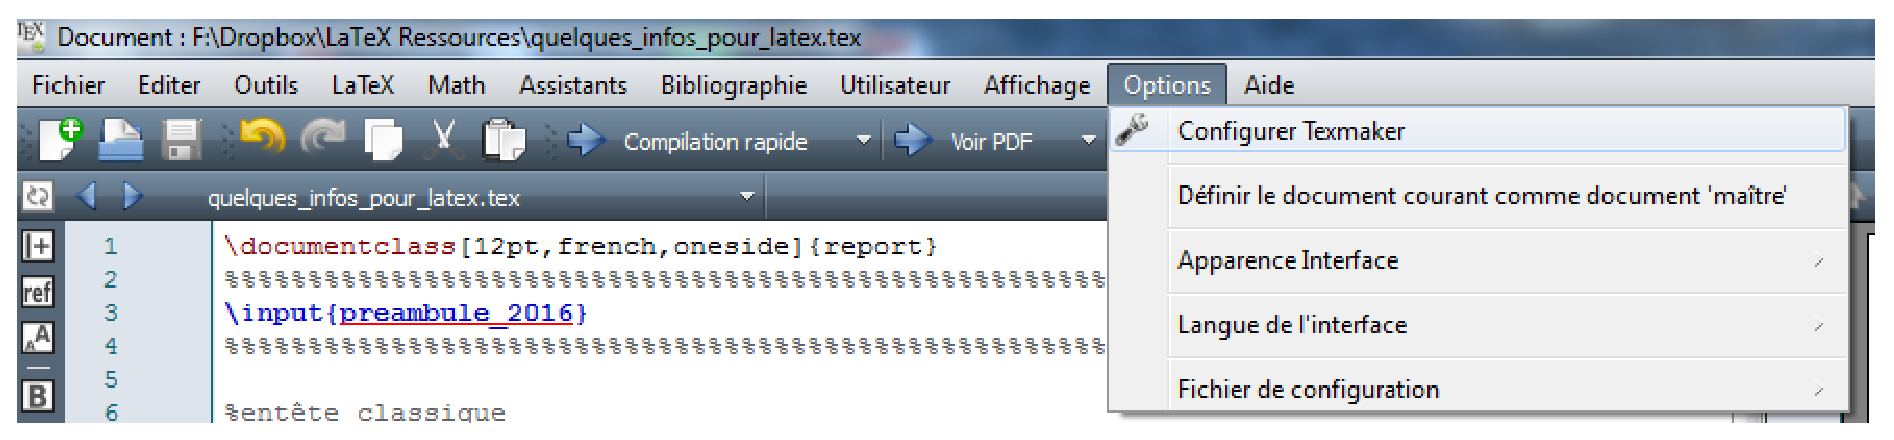
\includegraphics[width=0.8\textwidth]{installation/Capture1}
\end{center}

$\star$ On affiche l'écran suivant en choisissant \og Commandes \fg{} dans la barre gauche de la fenêtre qui vient de s'ouvrir.

On clique ensuite sur \og Afficher Pdf interne \fg{} et on coche \og Intégré à la fenêtre \fg{} :

\begin{center}
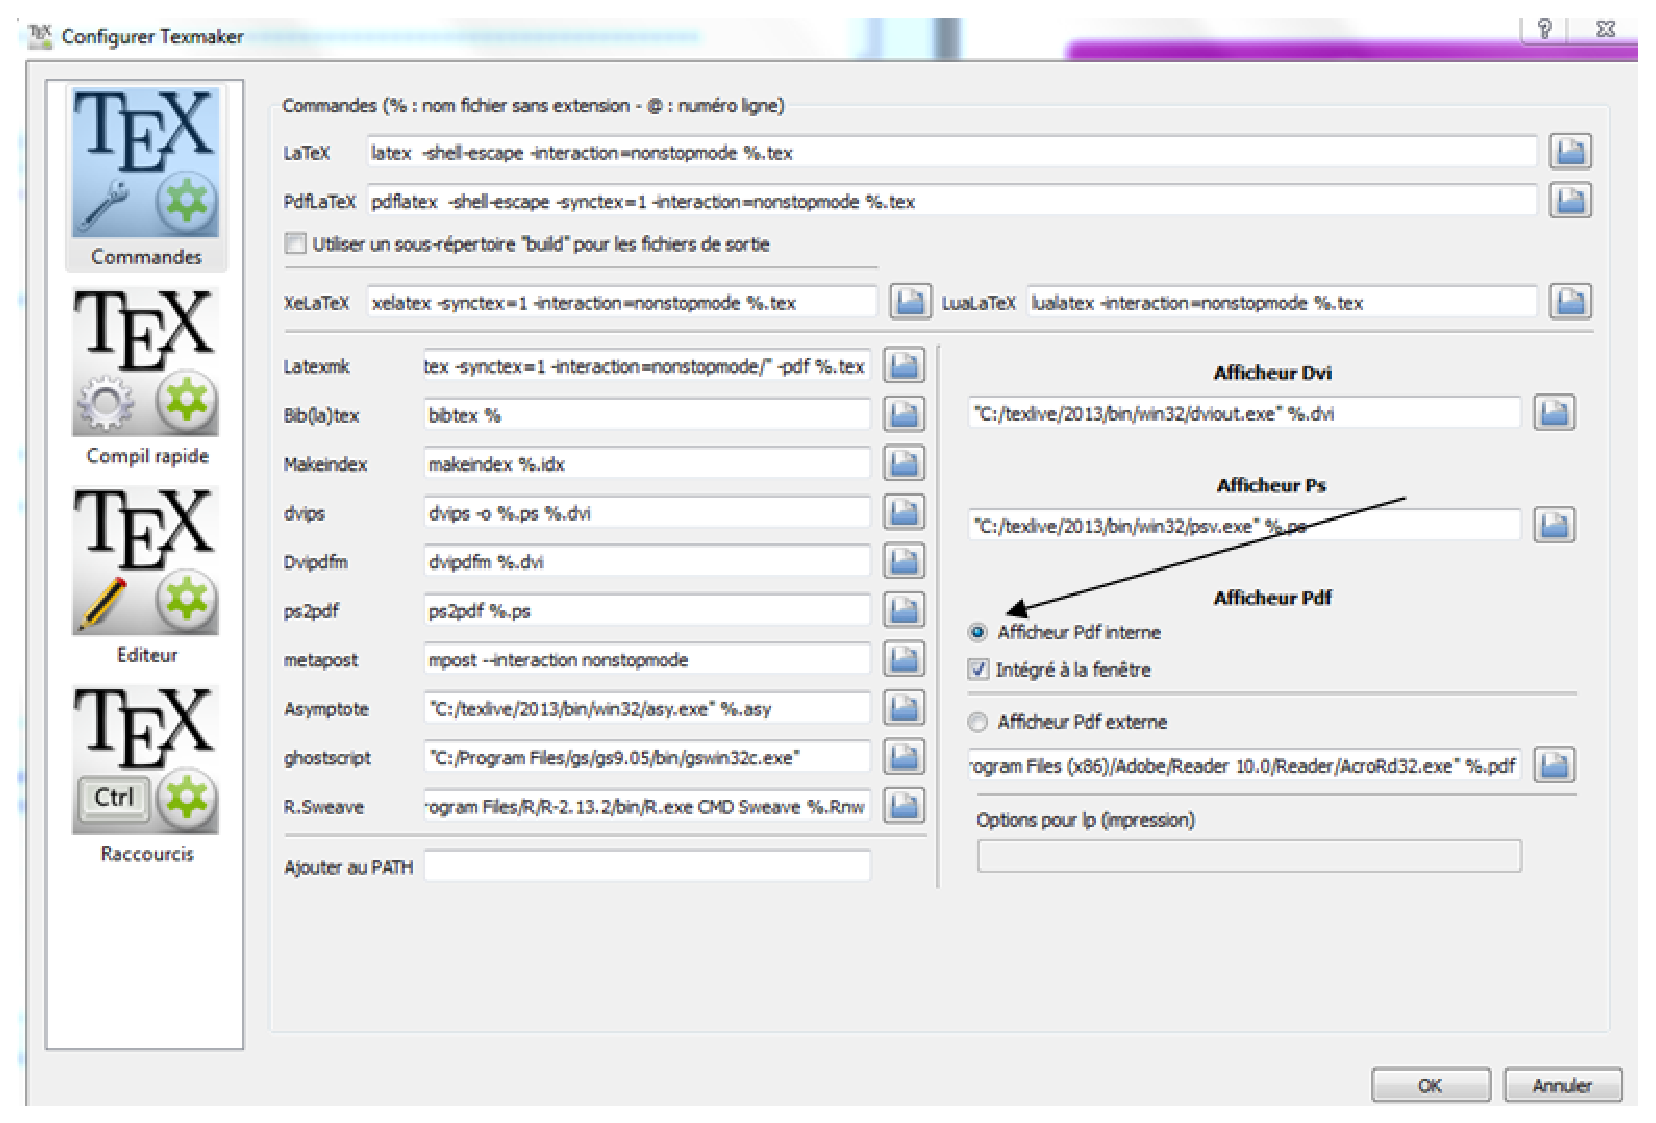
\includegraphics[width=0.8\textwidth]{installation/Capture2}
\end{center}

On valide en cliquant sur OK.

$\star$ Il suffit, pour terminer, de cocher sur \og Pdf Viewer\fg{} en bas à gauche :

\begin{center}
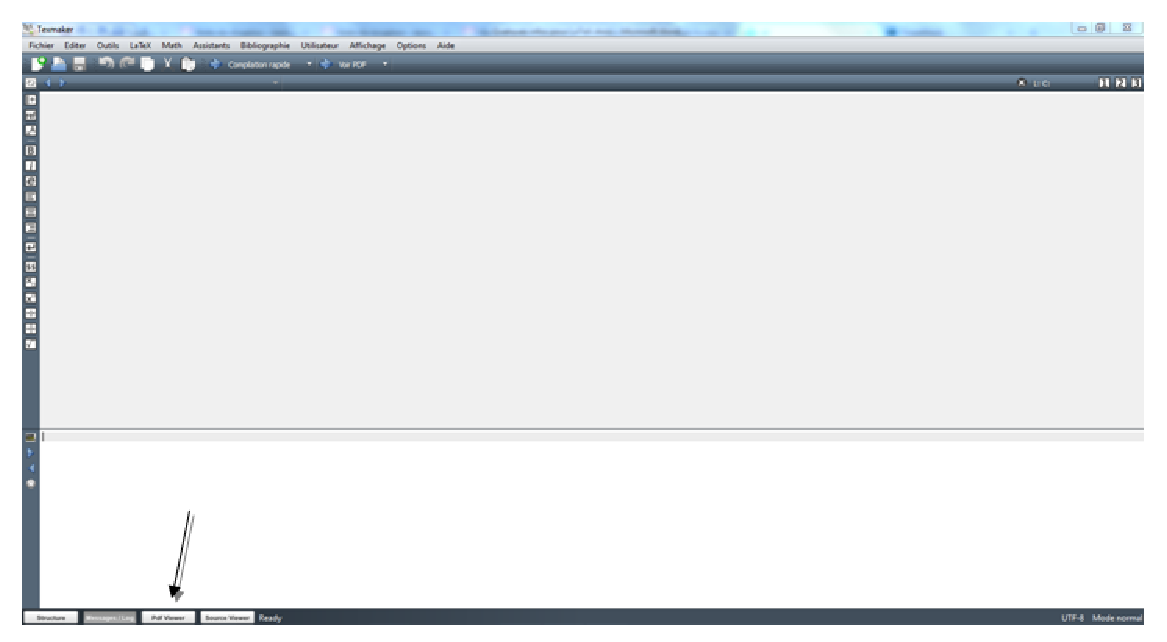
\includegraphics[width=0.8\textwidth]{installation/Capture}
\end{center}

\section{Personnalisation de TexMaker}

$\star$ Dans le menu \og Utilisateur\fg{},

\begin{itemize}

\item on peut créer des balises,

\item ajouter des commandes,

\item ajouter des termes au \og dictionnaire\fg{} initial reconnu par le logiciel qu'il utilise pour effectuer de l'auto-complétion.

\end{itemize}

$\star$ Dans le menu \og Options \fg{}, en cliquant sur\og Configurer Texmaker \fg{}, 

\begin{itemize}
\item on peut choisir le système d'encodage de l'éditeur

\begin{center}
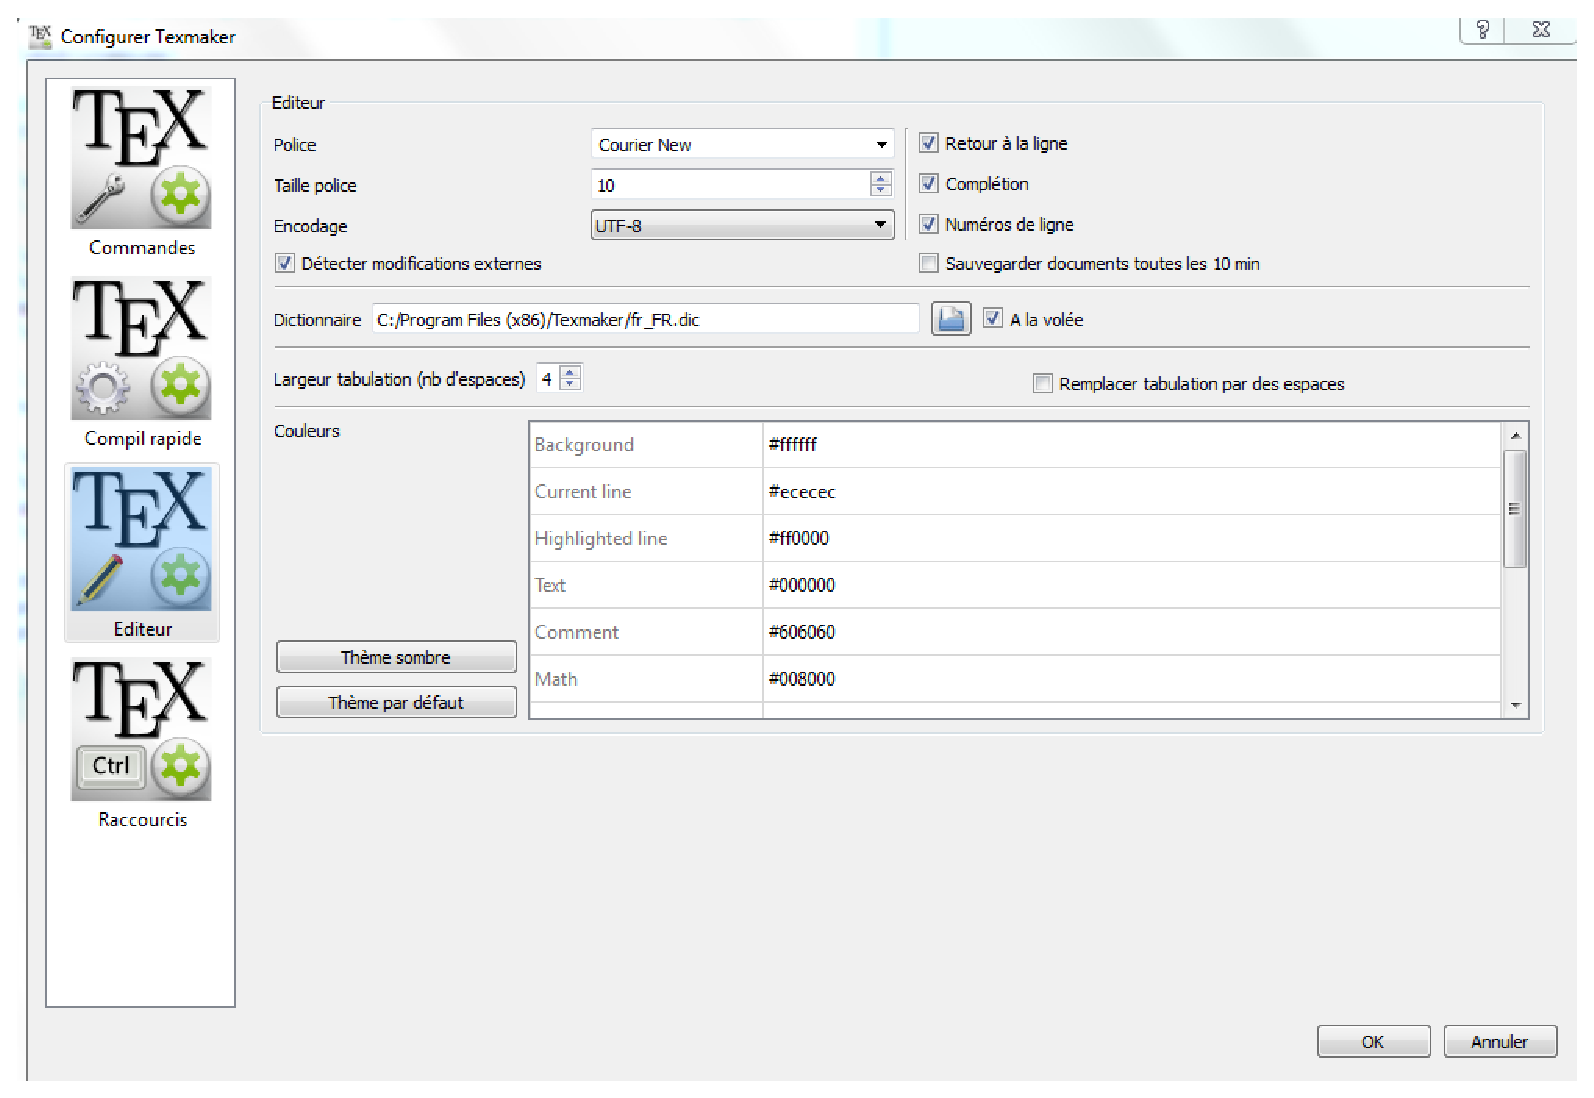
\includegraphics[width=0.5\linewidth]{installation/editeur_texmaker}
\end{center}

\item ainsi que la méthode de compilation (accessible par la touche \touche{F1})

\begin{center}
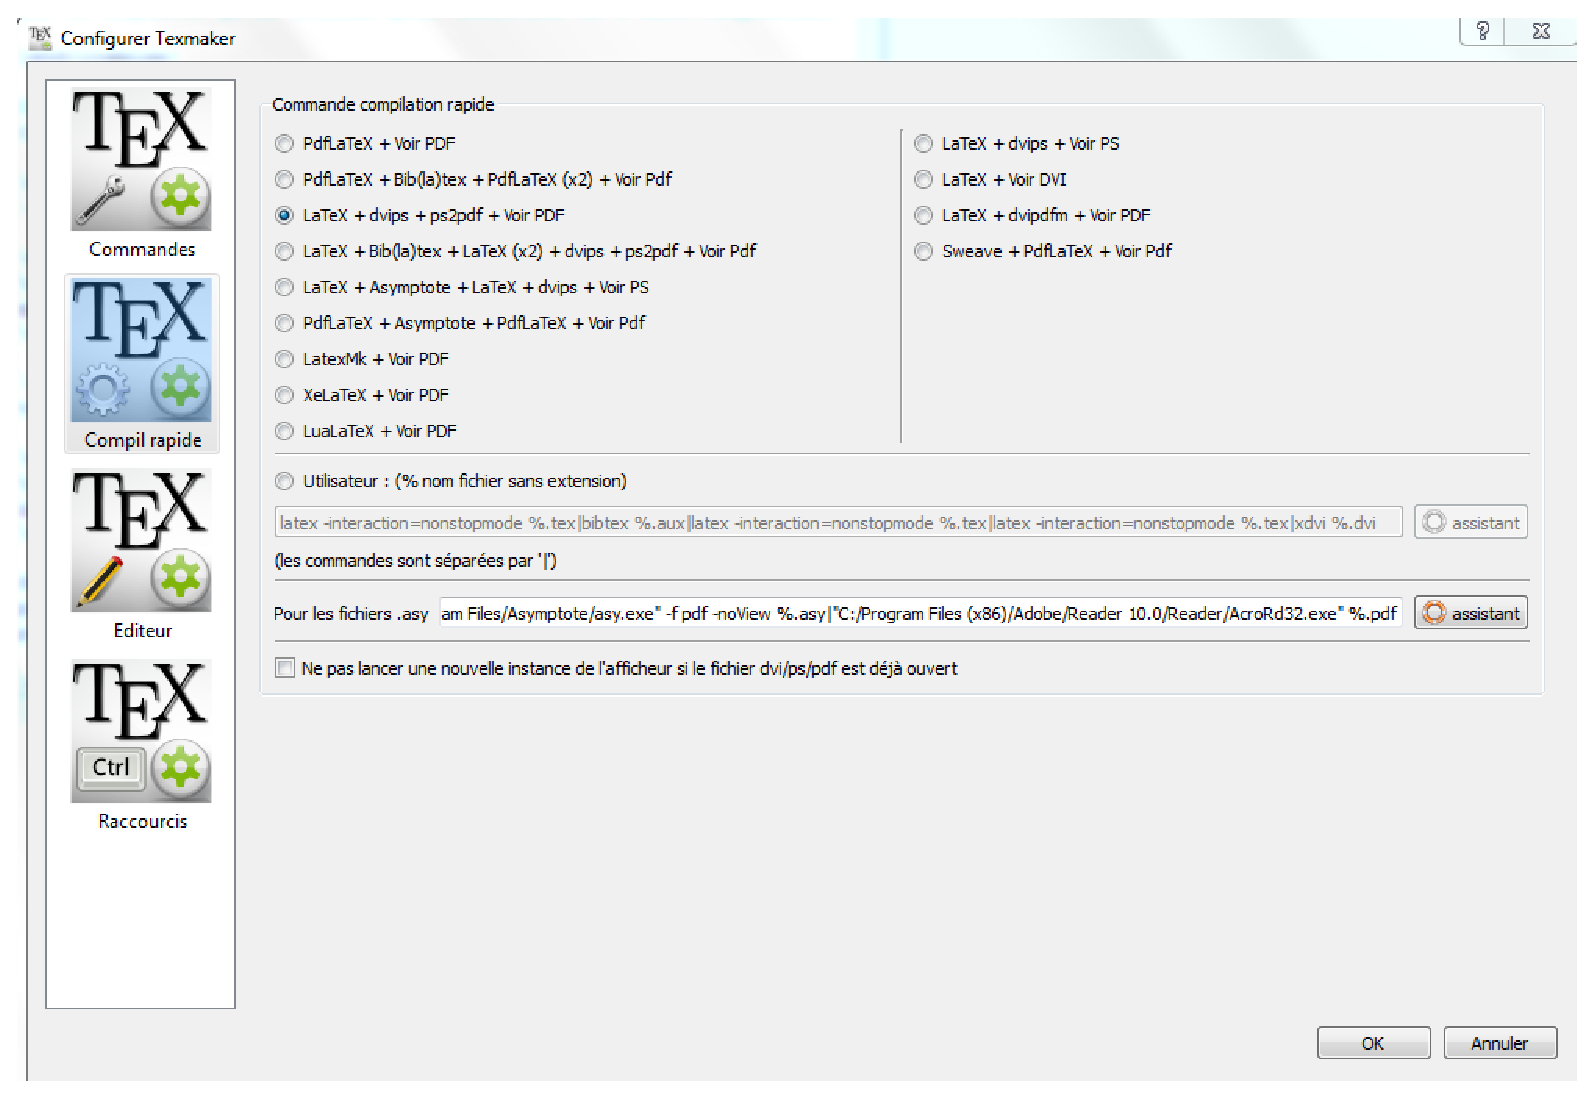
\includegraphics[width=0.5\linewidth]{installation/compil_texmaker}
\end{center}

Si le document final doit contenir des figures PSTricks et TikZ, préférez la méthode de compilation de la capture d'écran précédente.

\end{itemize}

\section{Installer un nouveau package non présent dans la distribution}

\subsection{\og À la main \fg{} }

Il existe plusieurs méthodes d'installation d'un  package avec LaTeX. J'ai sélectionné pour vous les deux plus faciles à mon sens. Elles devraient vous permettre d'utiliser la quasi-totalité des packages.

Les deux méthodes développées ici diffèrent légèrement, suivant que votre package est un fichier .ins ou .sty.

Dans de rares cas, les packages sont fournis sous d'autres extensions, mais ils sont alors accompagnés d'un fichier README vous guidant lors de leur installation.

\subsubsection{Les packages en .sty, méthode simple}

Si votre \jargon{package} est de la forme \verb~nom_de_package.sty~, rien de plus simple pour l'utiliser : il suffit de le copier dans le dossier contenant votre source .tex. Lorsque votre distribution compilera le fichier .tex, elle recherchera dans ce dossier les fichiers .sty des packages manquants, et le tour sera joué.

Résumons, la commande \verb~\usepackage{nom_de_package}~ demande à LaTeX d'utiliser un \jargon{package} installé ou, s'il ne l'est pas, d'aller chercher le fichier \verb~nom_de_package.sty~ dans le dossier de travail.

Simple, n'est-ce pas ?

Mais si l'on veut pouvoir réutiliser ce même \jargon{package} pour d'autres documents sans avoir à la copier dans le dossier de travail, on le copiera dans le dossier du PC contenant tous les \jargon{packages} :

\begin{enumerate}
\item Sur mon installation, il s'agit du répertoire :

\begin{enumerate}
\item \verb~C:\texlive\2013\texmf-dist\tex\latex~ pour mon pc sous Windows 7

\item \verb~/usr/local/texlive/2013/texmf-dist/tex/latex~ pour mon netbook sous Linux

\end{enumerate}

\item Il faut ensuite demander à la distribution installée de prendre en compte cet ajout :

\begin{enumerate}
\item Sous Windows

Lancer \og Tex Live Manager\fg{}, puis dans le menu \og Actions\fg{}, cliquer sur \og Update filename database\fg{}

OU

Lancer l'invite de commandes et taper \og texhash\fg{} (sans les guillemets\dots), puis valider.

\item Sous Linux

Lancer un terminal en administrateur et taper \og texhash\fg{} (sans les guillemets), puis valider.

\end{enumerate}

\end{enumerate}

\subsubsection{Les packages en .ins, méthode en deux temps}

Les \jargon{packages} contenus dans un fichier .ins doivent être traités en deux étapes. 

Premièrement, mettez votre fichier \verb~nom_de_package.ins~ dans un répertoire et compilez-le (c'est-à-dire, lancer la commande \verb~latex nom_de_package.ins~ en ligne de commandes) : il génèrera un fichier \verb~nom_de_package.sty~.

Ce fichier \verb~nom_de_package.sty~ doit être traité selon le processus développé dans le paragraphe \og Les packages en .sty, méthode simple \fg{}.



\subsection{Vérifier si un package est présent dans la distribution avec TeX Live Manager}

On lance Tex Live Manager et on voit alors apparaître la liste de tous les \jargon{packages} présents dans la distribution.

\begin{center}
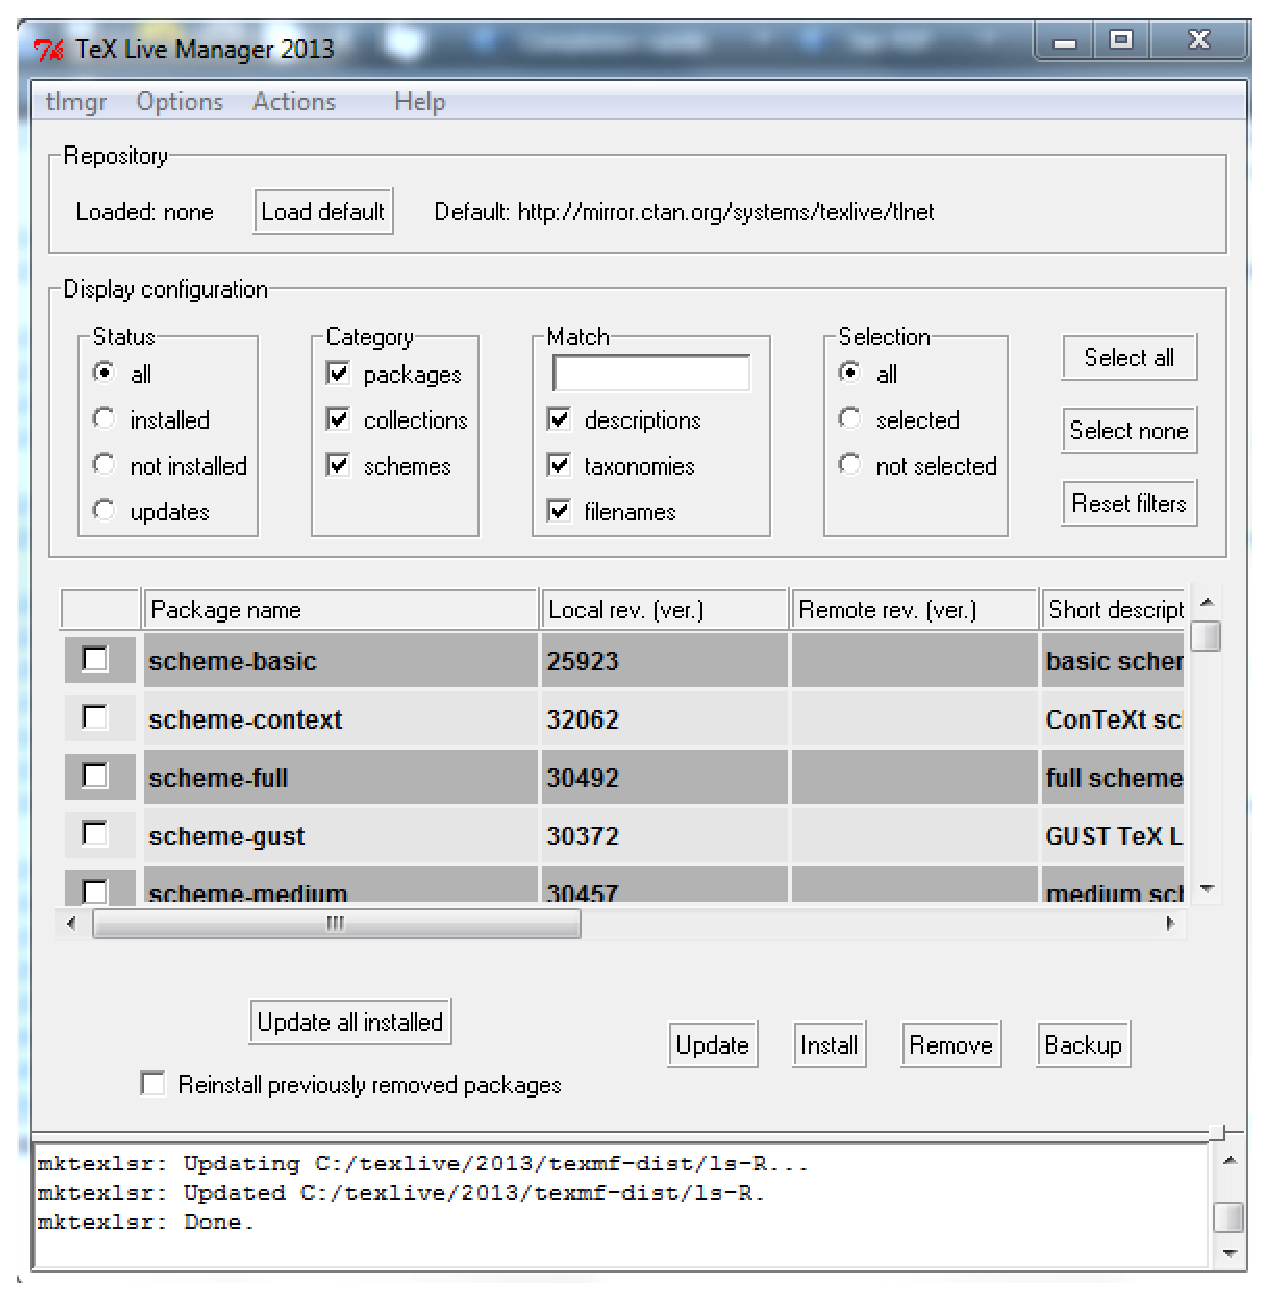
\includegraphics[width=0.6\textwidth]{installation/Capture3}
\end{center}


On peut également utiliser la ligne \og Match \fg{} en tapant les premières lettres du nom de \jargon{package} cherché pour accélérer la recherche.

\section{Sites sur lesquels on trouve des documents écrits avec \LaTeX}

$\star$ Parmi les sites sur lesquels on trouve des exercices de Mathématiques écrits avec \LaTeX, on peut citer \href{http://www.sesamath.net/}{Sesamath} dont les manuels pour le lycée utilisent \LaTeX, ou l'incontournable site de l'\href{http://www.apmep.fr/}{APMEP} avec sa section de sujets d'annales pour le brevet, le bac, le bts etc.

$\star$ Et parmi les très nombreux sites sur lesquels on trouve de la documentation sur l'utilisation de \LaTeX{} orientée \og Mathématiques \fg{}, on peut citer :

\begin{itemize}
\item la \href{http://math.univ-lyon1.fr/irem/spip.php?article340}{section dédiée} sur le site de l'Irem de l'académie de Lyon qui contient une brochure intitulée \og 	
LaTeX\dots pour le prof de maths ! \fg{} ,

\item le site \href{http://www.xm1math.net/}{xm1math} de Pascal Brachet (déjà cité plus tôt),

\item le site \href{http://math.et.info.free.fr/}{math.et.info} avec sa rubrique sur TikZ (très utile pour les figures et graphiques (voir le chapitre \ref{graph})),

\item le site \href{http://altermundus.fr/}{altermundus} qui contient de l'aide pour l'utilisation de TikZ et TkZ pour les graphiques et figures (voir le chapitre \ref{graph}),

\item et le site \href{http://www.texample.net/tikz/examples/}{texample.net} sur lequel on retrouve énormément de figures créées avec TikZ.

\end{itemize}


\section{Logiciels ou sites permettant d'extraire du code \LaTeX}

$\star$ Certains logiciels permettent d'exporter dans un format utilisable par \LaTeX{} les graphiques créés.

C'est le cas d'\textbf{Algobox}, de \textbf{Geogebra}, de \textbf{PdfAdd}, qui permet de créer les graphiques ci-dessous, en générant du code Asymptote (ou \LaTeX{} pour les tableaux de variations/signes) qu'il suffit de copier/coller dans son document \LaTeX{} :

\begin{center}
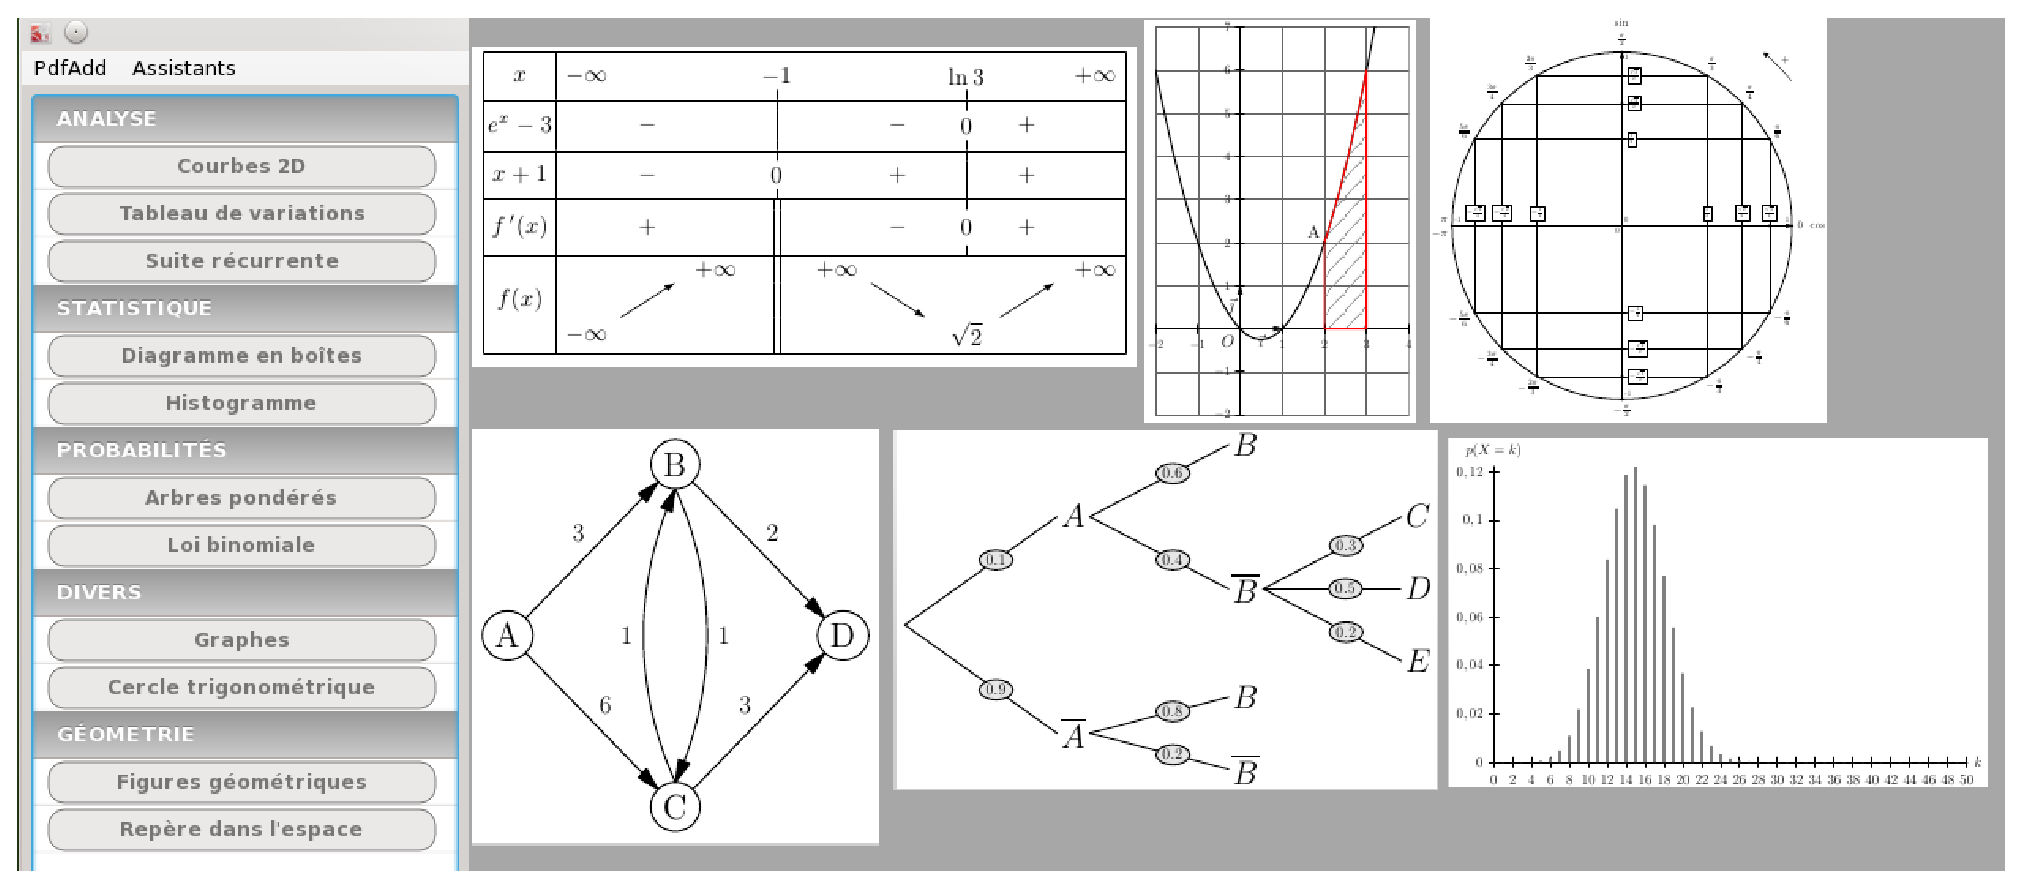
\includegraphics[width=0.7\textwidth]{installation/pdfadd}
\end{center}

C'est également le cas de \textbf{Pst+}, qui permet de créer les graphiques ci-dessous, en générant du code \LaTeX/PSTricks qu'il suffit de copier/coller dans son document \LaTeX{} :

\begin{center}
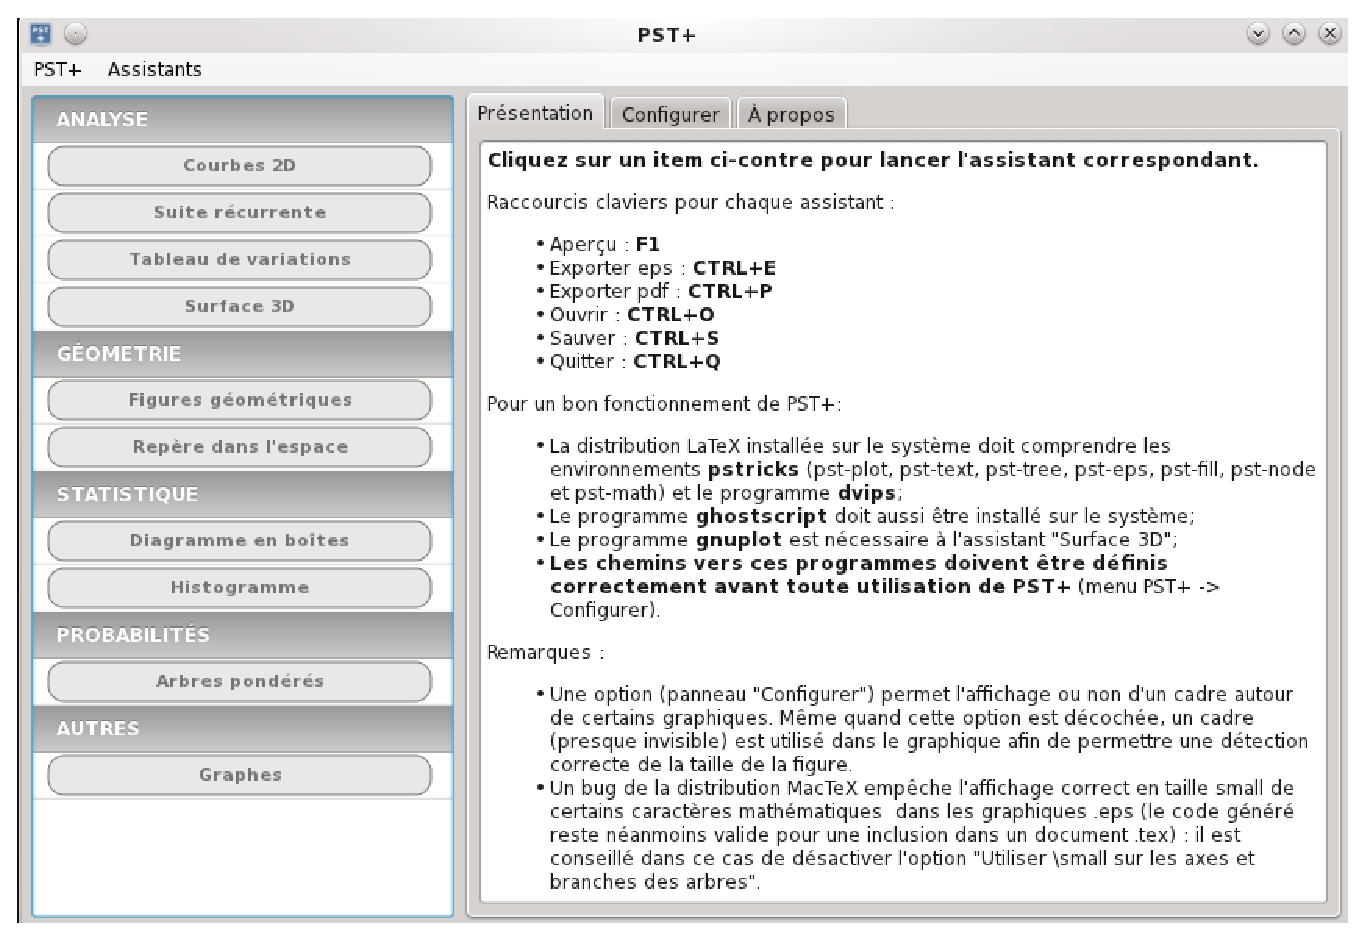
\includegraphics[width=0.7\textwidth]{installation/pstplus}
\end{center}

$\star$ On peut également intégrer du code \LaTeX{} dans la plupart des blogs, ou directement dans une zone graphique du logiciel \textbf{Geogebra}.

$\star$ Sur le site \href{http://math.et.info.free.fr/}{math.et.info}, on peut créer des tableaux de variations et des arbres pondérés, puis récupérer le code TikZ à copier/coller dans le document \LaTeX{}.